\documentclass[12pt,a4paper, french]{article}
\usepackage{natbib}         % Pour la bibliographie
\usepackage{url}            % Pour citer les adresses web
\usepackage[T1]{fontenc}    % Encodage des accents
\usepackage[utf8]{inputenc} % Lui aussi
\usepackage{babel} % Pour la traduction française

\usepackage{graphicx}
\usepackage{svg}
\graphicspath{ {./src/} }

% Mettez votre titre et votre nom ci-après
\title{Rapport de TIPE Sup \\
Reconnaissance vocale lors d'appel d'urgence grâce à un réseau de neurones}
\author{Tran-Thuong Tien-Thinh, MPSIA, 2020-2021}
\date{}

\begin{document}

\maketitle

\begin{abstract}
D'après les chiffres du ministère de la Santé, il y a plus de 31 millions d'appels d'urgence par an. Ces appels sont répartis sur 103 centres de plus en plus sollicités. Alors que les recommandations fixent un taux de 90\% de réponses en moins de 60 secondes, seul 69\% des appels étaient décrochés dans la minute.  

Afin de répondre à ce problème, nous nous proposons d'étudier une intelligence artificielle capable de faire de la reconnaissance vocale, pour alléger le travail des opérateurs d'appel d'urgence.
\end{abstract}

\section*{Problématique retenue}
\noindent\textit{INFORMATIQUE (Informatique Pratique)}

Il s’agit de concevoir un réseau de neurones capable de reconnaitre la voix, retranscrire ce qui est dit et de classer le niveau d'urgence d'un appel.

\section*{Objectif TIPE du candidat}
\begin{enumerate}
    \item Faire un réseau de neurones qui converge grâce à l’algorithme du gradient
    \item Améliorer la vitesse d'entrainement grâce à des optimizers basés sur la descente de gradient
    \item Essayer ce réseau sur la base de données du MNIST pour reconnaitre des chiffres
    \item Utiliser le transfert d'apprentissage pour reconnaître le nom de la personne qui a été prononcé dans un audio
\end{enumerate}

\section{Un réseau de neurones imitant l'opérateur XOR}
La difficulté de l'opérateur XOR est qu'il n'effectue pas une classification linéaire entre les deux entrées :
\begin{center}
\begin{tabular}{ |c|c||c|   }
 \hline
 \multicolumn{3}{|c|}{Tableau de l'opérateur XOR} \\
 \hline
 Entrée 1 & Entrée 2 & Sortie\\
 \hline
 0 & 0 & 0\\
 1 & 0 & 1\\
 0 & 1 & 1\\
 1 & 1 & 0\\
 \hline
\end{tabular}
\end{center}

\subsection{Réseaux de neurones}
Il est possible de démontrer que la taille minimum du réseau de neurone est 2 entrées, 2 neuronnes cachées et 1 neurone en sortie.  

Pour améliorer la vitesse d'apprentissage il est possible d'utiliser des fonctions d'activation permettant de normaliser les sorties de chaque neurone entre $[0, 1]$, comme la fonction \textit{sigmoïde}.
\begin{equation}
	\sigma(x) = \frac{1}{1+e^{-x}}
\end{equation}

\begin{center}
    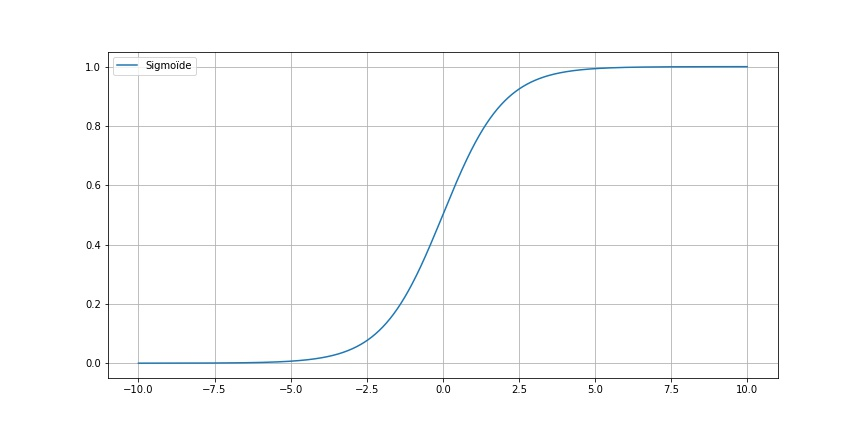
\includegraphics[height=4cm]{1-trace sigmoid.jpg} \\
    Courbe de la fonction d'activation sigmoïde
\end{center}


\subsection{Apprentissage}
L'apprentissage des poids sur chaque neurone, se fait en calculant l'erreur, et en utilisant la rétropropagation. On peut calculer la différence à appliquer au poids par rapport à l'erreur $\frac{d_{erreur}}{d_w}$ grâce à la descente de gradient.

\begin{equation}
	\frac{d_{erreur}}{d_{poids}} = 
		\frac{d_{erreur}}{d_{\sigma(sortie)}} 
		\times 
		\frac{d_{\sigma(sortie)}}{d_{sortie}} 
		\times 
		\frac{d_{sortie}}{d_{poids}}   
\end{equation}
\begin{equation}
	\frac{d_{erreur}}{d_{poids}} = 
		2(\sigma(sortie) - sortie_{cible})
		\times 
		\sigma'(sortie)
		\times 
		entree  
\end{equation}

\begin{center}
    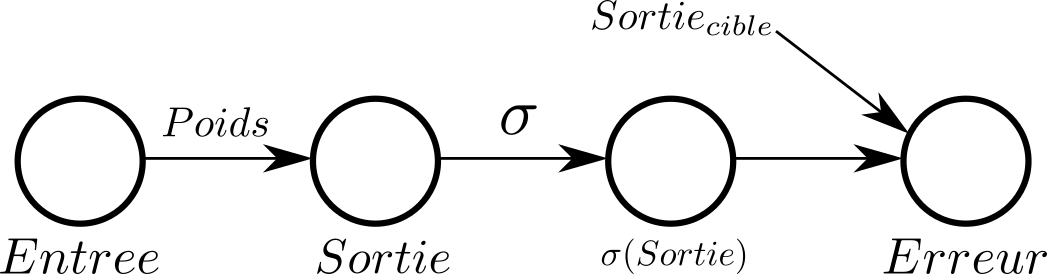
\includegraphics[width=10cm]{1-Neuronne backpropagation.png} \\
    Représentation du dernier neurone
\end{center}

\subsection{Resultats}
Le réseau de neurones indique bien les résultats associés au XOR :
\\
\noindent 
\textsf{
Les entrées [0, 0] donnent en sortie 0.03356776609399469 \\ 
Les entrées [1, 0] donnent en sortie 0.9295281916216991  \\
Les entrées [0, 1] donnent en sortie 0.9295281849281336  \\
Les entrées [1, 1] donnent en sortie 0.09395448088880454  \\
}

Le temps d'apprentrissage est cependant très long, il a pris près de 100 000 époques avant de converger vers un résultat d'erreur inférieur à 10\%.

\begin{center}
    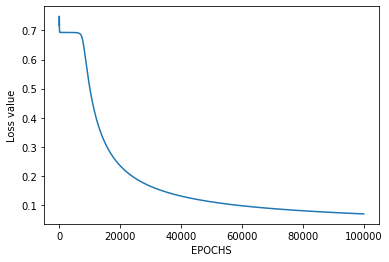
\includegraphics[width=7cm]{1-Courbe d'erreur d'apprentissage du XOR.png} \\
    Courbe d'erreur d'apprentissage du XOR
\end{center}

\section{Optimizers}
Une façon d'accélérer la vitesse d'apprentissage des neurones est l'utilisation des optimizers améliorant la descente de gradient simple.

\subsection{Regroupement des données par paquet (batch)}
Pour améliorer la vitesse d'apprentissage il est intéressant de grouper les données par paquet (batch) et de mettre à jour le poids des neurones après avoir évalué la sortie pour toutes les données d'un paquet. On réduit le nombre de mises à jour des poids, et on évite l'impact des données aberrantes.  

Afin de choisir rapidement la taille des paquets il est conseillé de procéder par dichotomie avec des paquets aléatoires de $\{64; 128; 256; 512\}$ données.

\subsection{Moment}
Le moment permet d'accentuer la modification des poids lorsque plusieurs données consécutives génèrent les mêmes modifications. Cela permet de varier le taux d'apprentissage (learning rate) en cohérence avec les données passées.

\begin{center}
    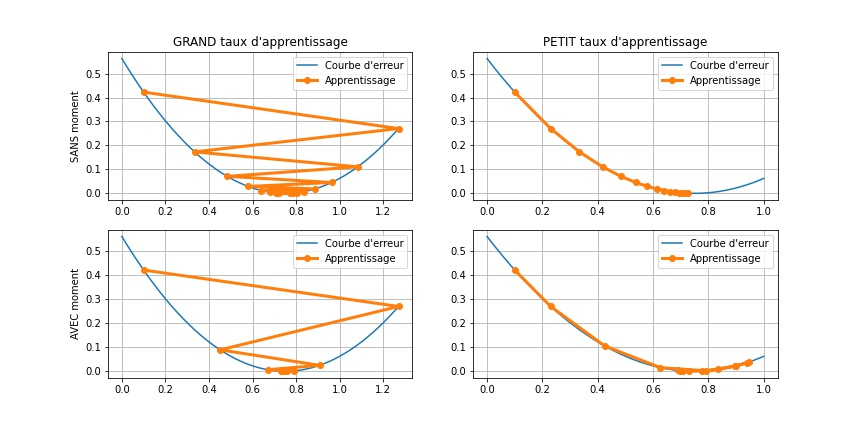
\includegraphics[width=12cm]{2-Moment VS sans Moment.jpg} \\
    Courbe d'erreur d'apprentissage d'un neurone sans puis avec moment
\end{center}

Au lieu de modifier directement le poids des neurones avec la formule :
\begin{equation}
	poids \leftarrow
	poids - taux_{apprentissage} \times d_{poids}
\end{equation}

On prend en compte les poids passées avec $\gamma = 0.5$ le taux de considération du moment précédent :
\begin{equation}
	d_{moment} \leftarrow 
	\gamma * d_{moment} + taux_{apprentissage} * d_{poids}
\end{equation}
\begin{equation}
	poids \leftarrow
	poids - d_{moment}
\end{equation}


Le moment permet également de résoudre des problèmes possédants des solutions locales non optimales au lieu d'y rester bloquer.

\begin{center}
    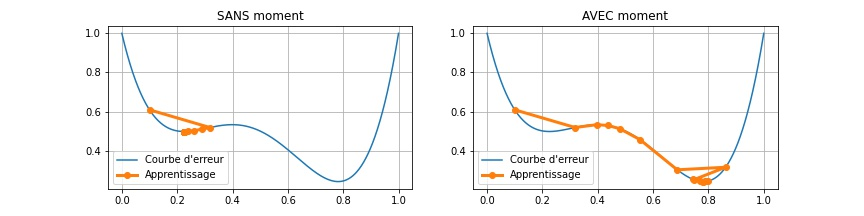
\includegraphics[width=12cm]{2-Moment remonte.jpg} \\
    Courbe d'erreur comportant un minimum local
\end{center}

\section{MNIST reconnaissance de chiffres écrits à la main}
Comme c'est un problème de classification avec $10$ classes différentes $[|0; 9|]$, il est plus intéressant d'utiliser la fonction d'activation \textit{softmax} :  
\begin{equation}
	\sigma(X)_i = \frac{e^{X_i}}{\sum_{j=0}^{9}{e^{X_j}}} 
	\quad \textrm{avec} \quad
	\textrm{X la matrice colonne des 10 sorties}
\end{equation}

\subsection{Résultat}

\begin{center}
    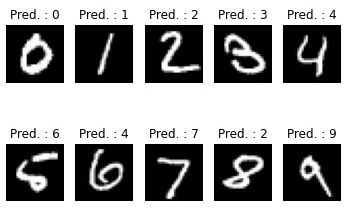
\includegraphics[width=7cm]{3-Prediction.jpg} \\
    Prediction : 7 bonnes réponses sur 10
\end{center}

On obtient plus de 63\% de bonne réponses sur les données de test, mais il a fallu l'entrainer 1 500 époques (50 minutes environ) d'apprentissage.

\begin{center}
    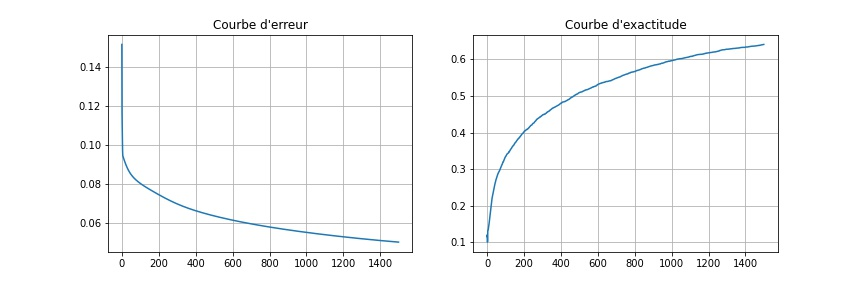
\includegraphics[width=9cm]{3-apprentissage.jpg} \\
    Courbes d'apprentissage
\end{center}

J'ai donc appliqué l'optimizer avec le moment sur les 50 premières époques. On remarque un apprentissage plus rapide au début de l'apprentissage.

\begin{center}
    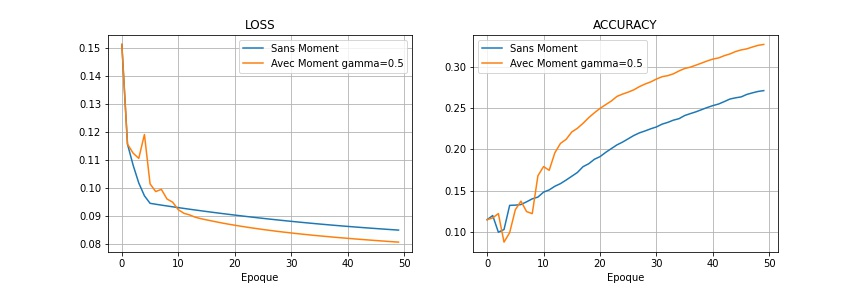
\includegraphics[width=12cm]{3-MNIST moment vs sans.jpg} \\
    Amélioration de l'apprentissage du réseau de neurones grâce au moment
\end{center}

\section{Classification d'audio }
Mon but est de classifier des séquences audio. J'ai donc essayé de faire un réseau de neurones capable de reconnaître les noms de mes professeurs \{"Bensal", "Châteaux", "Gayout", "Le Grandic", "Mistler", "Schuschu"\}. Pour cela j'ai décomposé l'audio avec la transformée de Fourier .

\begin{center}
    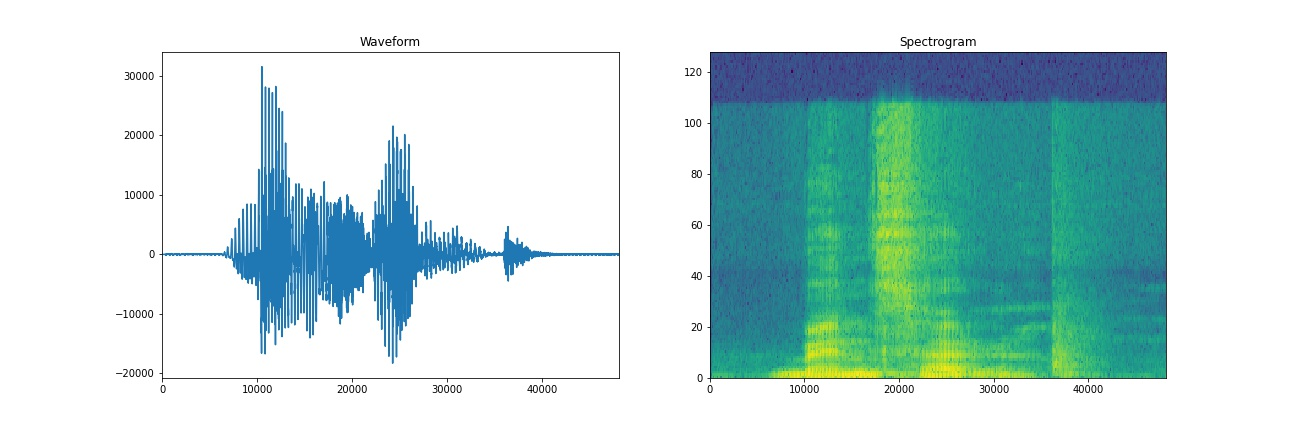
\includegraphics[width=13cm]{4-Audio Bensaal.jpg} \\
    Un audio "Bensal" et sa décomposition \textit{Short-time Fourier transform}
\end{center}

\subsection{Transfert d'apprentissage}
\textit{Cette section utilise la librairie Tensorflow pour la création et l'entrainement des réseaux de neurones.}  
  
J'ai entrainé un modèle sur une base de données de Google avec les mots \{"down", "go", "left", "no", "right", "stop", "up", "yes"\} afin de l'entrainer à reconnaître des sons caractéristiques avec un grand nombre de données. Le modèle entrainé, j'en ai extrait les premières couches de neurones et dont j'ai fixé les poids. J'ai ensuite rajouté des neurones permettant de reconnaitre les noms qui sont prononcés à partir des sons caractéristiques.
\begin{center}
    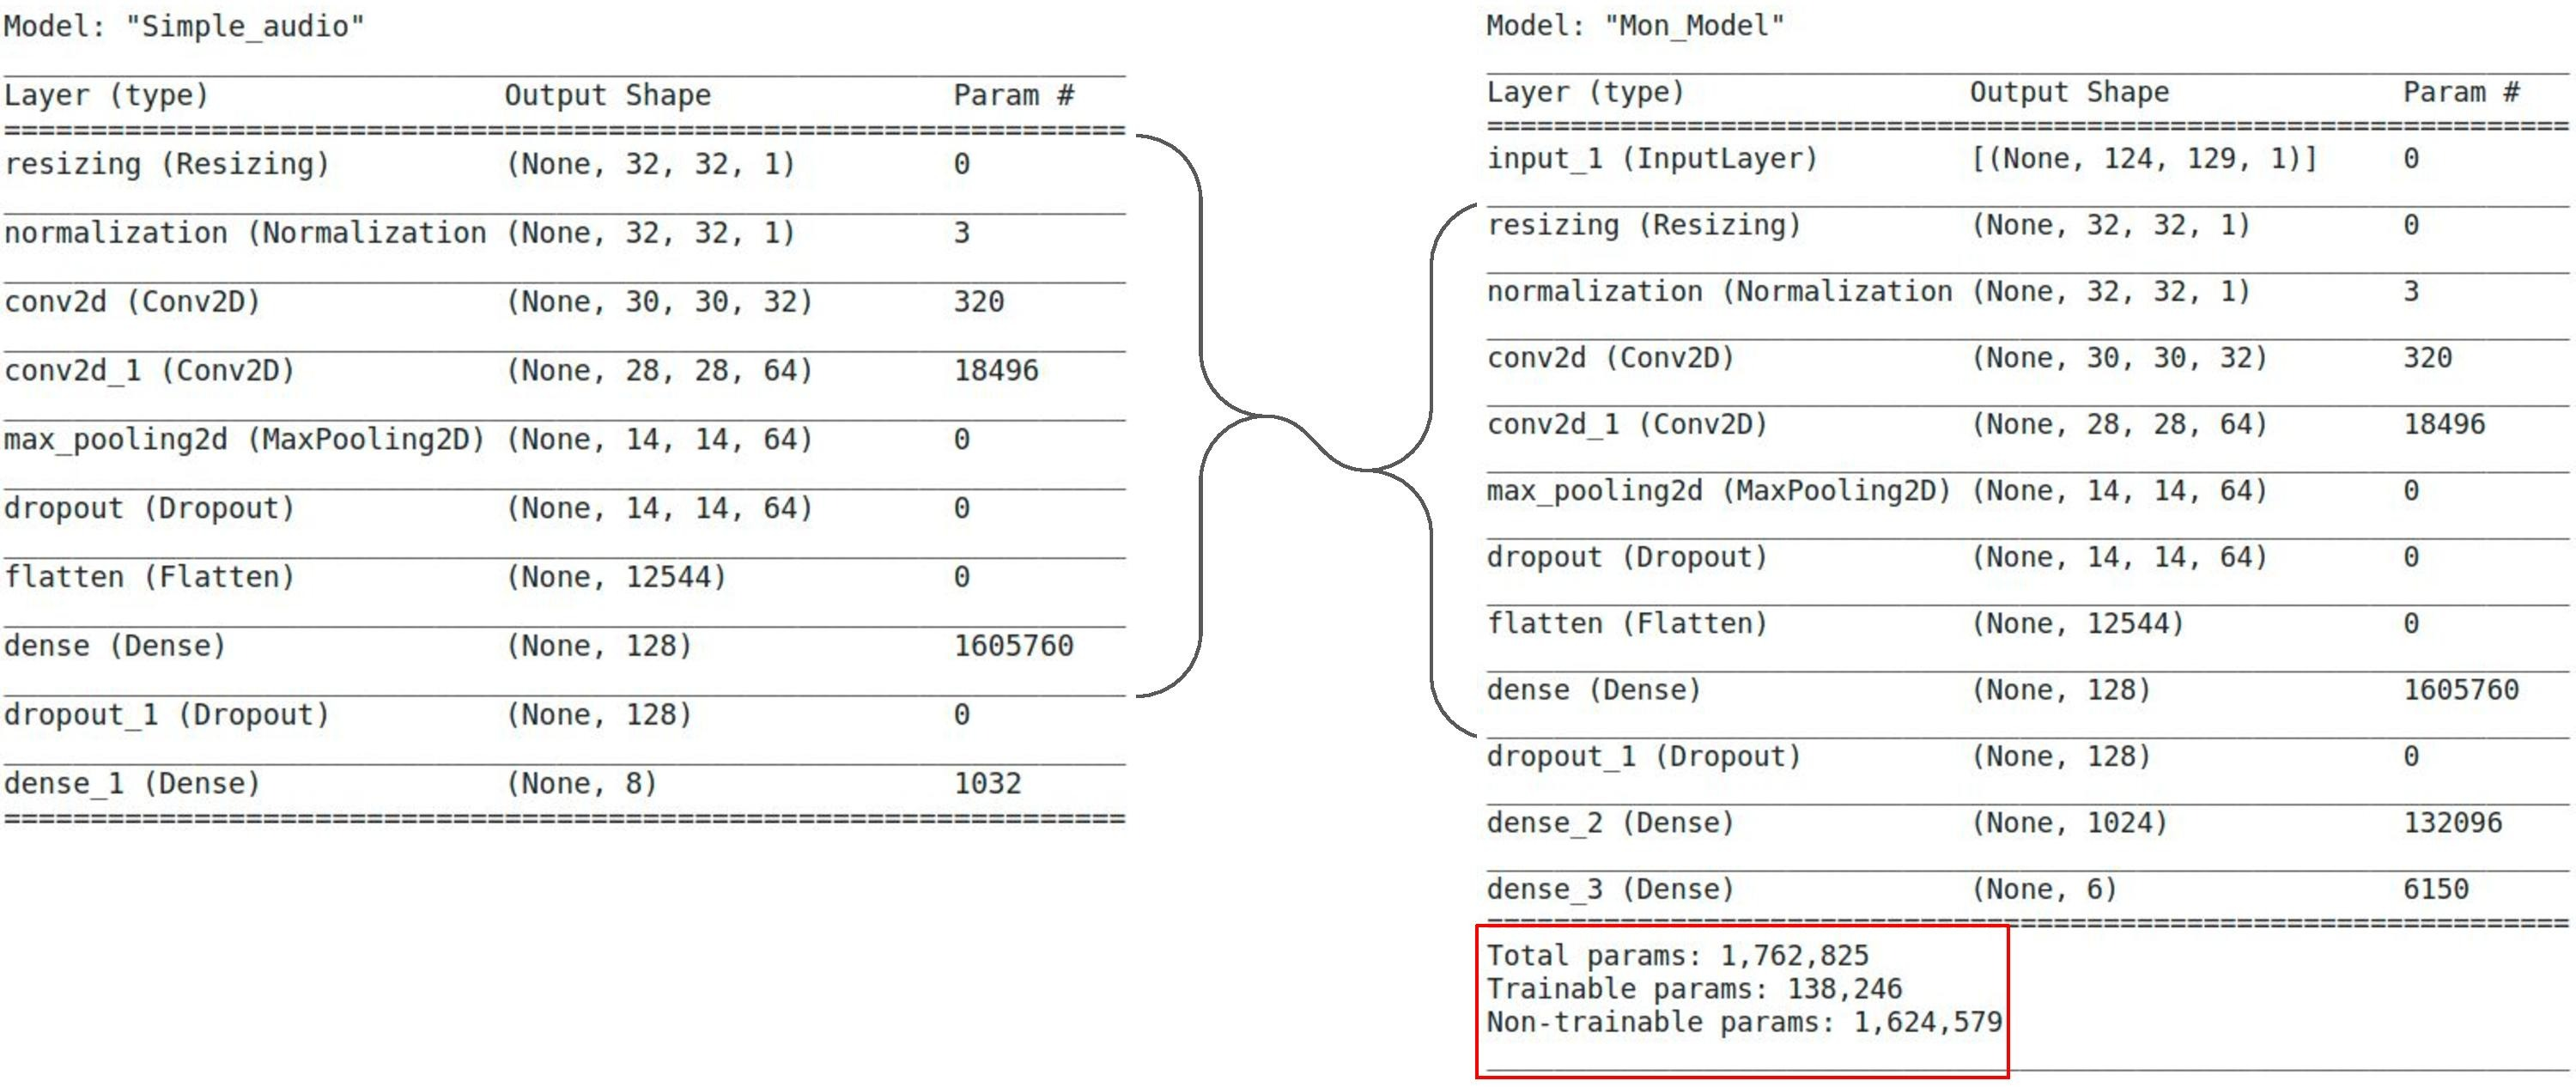
\includegraphics[width=12cm]{4-Transfert Learning.jpg} \\
    Transfert des couches de \textit{Simple audio} vers \textit{Mon model}
\end{center}

\subsection{Augmentation de données}
J'ai enregistré Agathe et moi en train de dire les noms 8 fois. Mais il fallait beaucoup plus de données, j'ai donc fait de l'augmentation de données (petites modifications des données permettant d'avoir des données différentes) :  
\begin{enumerate}
	\item Ajout de bruit $\times 4$
	\item Modulation de la voix (grave, aigu) $\times 4$
	\item Modulation de la vitesse du son $\times 4$
	\item Découpage du son $\times 4$
\end{enumerate}
Ce qui me permet de me retrouver avec $4^4 = 256$ fois plus de données différentes. Ainsi je me retrouve avec $256 \times 8 \times 2 = 4096$ audios.

\subsection{Résultat}
Les résultat sont concluants, il y a plus de 80\% de bonnes réponses lorsque c'est Agathe ou moi qui testons. Ce taux d'exactitude est réduit en fonction de la voix et l'intonation de la personne qui teste le modèle. 

\begin{center}
    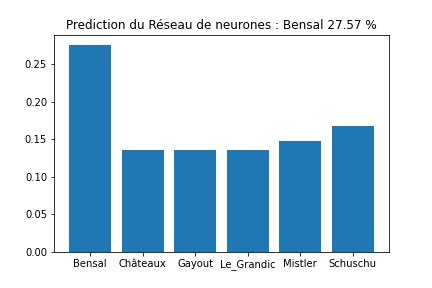
\includegraphics[width=8cm]{4-Resultat Bensal.jpg} \\
    Prediction pour un audio où "Bensal" a été prononcé
\end{center}

\section*{Annexes}
Tous mes codes : github.com/tttienthinh/4Tipe


\end{document}